\documentclass[
	fontsize = 10.0pt,
	a4paper,
	parskip = half*,
	twoside,	% do not middle align the page numbers
]{scrartcl}

% \usepackage{showframe}			% show page margins
\usepackage{xcolor}
\usepackage{graphicx}

\usepackage[latin1]{inputenc}	% mutated vowels
\usepackage{tabularx}
% set the page margins (space left/right/top/bottom) of the page
\usepackage	[	left	= 20mm,
				right	= 20mm,
				top		= 30mm,
				bottom	= 30mm
			]{geometry}


% TABLES / ARRAYS
\renewcommand{\arraystretch}{1.5}			% vertical distance between entries
\usepackage{float}
\usepackage{multirow}

\newcommand\CVname{John Doe Cat}
\newcommand\CVcitizenship{johndoeland}
\newcommand\CVphonenumber{(+43) 664123456789}
\newcommand\CVbirthdate{01/02 1900}
\newcommand\CVmail{john@doe.com}
\newcommand\CVaddress{john-doe street 13 (Johndoe country)}

% colorbar settings
\newcommand{\hlinewidth}{0.5mm}
\newcommand{\hlinelength}{150mm}
\newcommand{\hlinecolor}{black!25}
\newcommand{\hlinevskip}{-4.0mm}

% vertical spacing between entries (work experience / educational entries)
\newcommand{\vskipEntries}{-5.0mm}

% horizontal space for the dates (educational, work experience etc.)
\newcommand{\hskipFirstColumn}{5.0cm}

\begin{document}
	\pagenumbering{arabic}

	{\fontsize{20pt}{17pt}\selectfont\scshape \CVname}

	\begin{table}[H]
		\begin{tabular}{ p{3cm} l l }		% table formatting
			\multirow{5}{*}{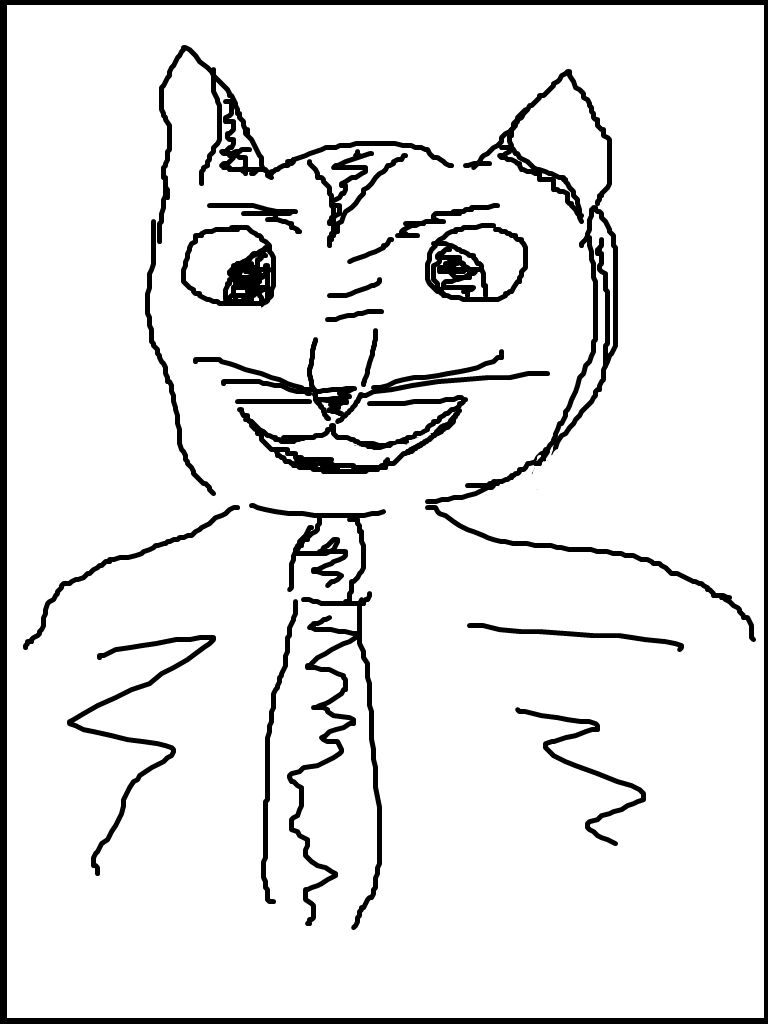
\includegraphics[height = 3.0cm]{cv_photo}}		&	\textbf{Citizenship}		&	\CVcitizenship	\\
																			&	\textbf{Telephone number}	&	\CVphonenumber	\\
																			&	\textbf{Date of birth}		&	\CVbirthdate	\\
																			&	\textbf{E-mail}				&	\CVmail			\\
																			&	\textbf{Address}			&	\CVaddress		\\
		\end{tabular}
	\end{table}%

	{\fontsize{20pt}{17pt}\selectfont\scshape Work Experience}
	\vskip \hlinevskip%
	\textcolor{\hlinecolor}{\rule{\hlinelength}{\hlinewidth}}

	\renewcommand{\arraystretch}{1.25}			% vertical distance between entries in the array
	\begin{table}[H]
		\begin{tabular}{ p{\hskipFirstColumn} l }		% table formatting
			September 2004 - June 2007		&	{\fontsize{14pt}{10pt}\selectfont\bfseries Cattamer}	\\
											&	\textbf{Cat Circus Lt.}									\\
											&	Comforting cats											\\
		\end{tabular}
	\end{table}%

	\vspace{\vskipEntries}

	\begin{table}[H]
		\begin{tabular}{ p{\hskipFirstColumn} l }		% table formatting
			March 2000 - December 2006		&	{\fontsize{14pt}{10pt}\selectfont\bfseries Dogtamer}	\\
											&	\textbf{Dog Taming Lt.}									\\
											&	Comforting dogs											\\
		\end{tabular}
	\end{table}%

	{\fontsize{20pt}{17pt}\selectfont\scshape General and Vocational Education}
	\renewcommand{\arraystretch}{1.25}			% vertical distance between entries
	\vskip \hlinevskip%
	\textcolor{\hlinecolor}{\rule{\hlinelength}{\hlinewidth}}

	\begin{table}[H]
		\begin{tabular}{ p{\hskipFirstColumn} l }		% table formatting
			April 1998 - December 2000		&	{\fontsize{10pt}{10pt}\selectfont\bfseries Catuniversity: Address 1/24K Catcity}	\\
											&	\textbf{Master of Cats}									\\
											&	Thesis: Cats Sleeping Pattern							\\
		\end{tabular}
	\end{table}%

	\vspace{\vskipEntries}

	\begin{table}[H]
		\begin{tabular}{ p{\hskipFirstColumn} l }		% table formatting
			April 1995 - December 1997		&	{\fontsize{10pt}{10pt}\selectfont\bfseries High School for cats: Address 1/24K}	\\
											&	\textbf{Cat Diploma}									\\
											&	Thesis: Coexistence of Cats and Dogs							\\
		\end{tabular}
	\end{table}%

	{\fontsize{20pt}{17pt}\selectfont\scshape Language Skills}
	\vskip \hlinevskip%
	\textcolor{\hlinecolor}{\rule{\hlinelength}{\hlinewidth}}

	\renewcommand{\arraystretch}{1.35}			% vertical distance between entries
	\begin{table}[H]
		\begin{tabular}{ l }
			\textbf{Catspeak} (Mother tongue), \textbf{Dogspeak} (excellent), \textbf{Spiderspeak} (basic)\\
		\end{tabular}
	\end{table}%

	{\fontsize{20pt}{17pt}\selectfont\scshape Digital Skills}
	\vskip \hlinevskip%
	\textcolor{\hlinecolor}{\rule{\hlinelength}{\hlinewidth}}

	\begin{table}[H]
		\begin{tabular}{ l}
			OfficeCat, MsDog, etc.
		\end{tabular}
	\end{table}%

	{\fontsize{20pt}{17pt}\selectfont\scshape Social Skills}
	\vskip \hlinevskip%
	\textcolor{\hlinecolor}{\rule{\hlinelength}{\hlinewidth}}

	\begin{table}[H]
		\begin{tabular}{ l}
			Excellent at playing with other cats.
		\end{tabular}
	\end{table}%

	\pagebreak	% break the page here

	{\fontsize{20pt}{17pt}\selectfont\scshape Volunteering}
	\vskip \hlinevskip%
	\textcolor{\hlinecolor}{\rule{\hlinelength}{\hlinewidth}}

	\begin{table}[H]
		\begin{tabular}{ p{\hskipFirstColumn} l }		% table formatting
			January 2001 - April 2005		&	{\fontsize{10pt}{10pt}\selectfont\bfseries Voluntary Worker at the Red Cat Cross}	\\
											&	Transporting sick cats																\\
		\end{tabular}
	\end{table}%

	\vspace{\vskipEntries}

	\begin{table}[H]
		\begin{tabular}{ p{\hskipFirstColumn} l }		% table formatting
			January 1995 - April 2000		&	{\fontsize{10pt}{10pt}\selectfont\bfseries Voluntary Worker at the Red Dog Cross}	\\
											&	Caring for sick dogs																\\
		\end{tabular}
	\end{table}%

\end{document}
